\begin{frame}{Motivation}
    How much of the difference between \texttt{n3fit} and \texttt{nnfit} can be explained by the minimisation methods? \\
    
    \vspace{3pt}

    \only<1>{
    \begin{figure}
        \centering
        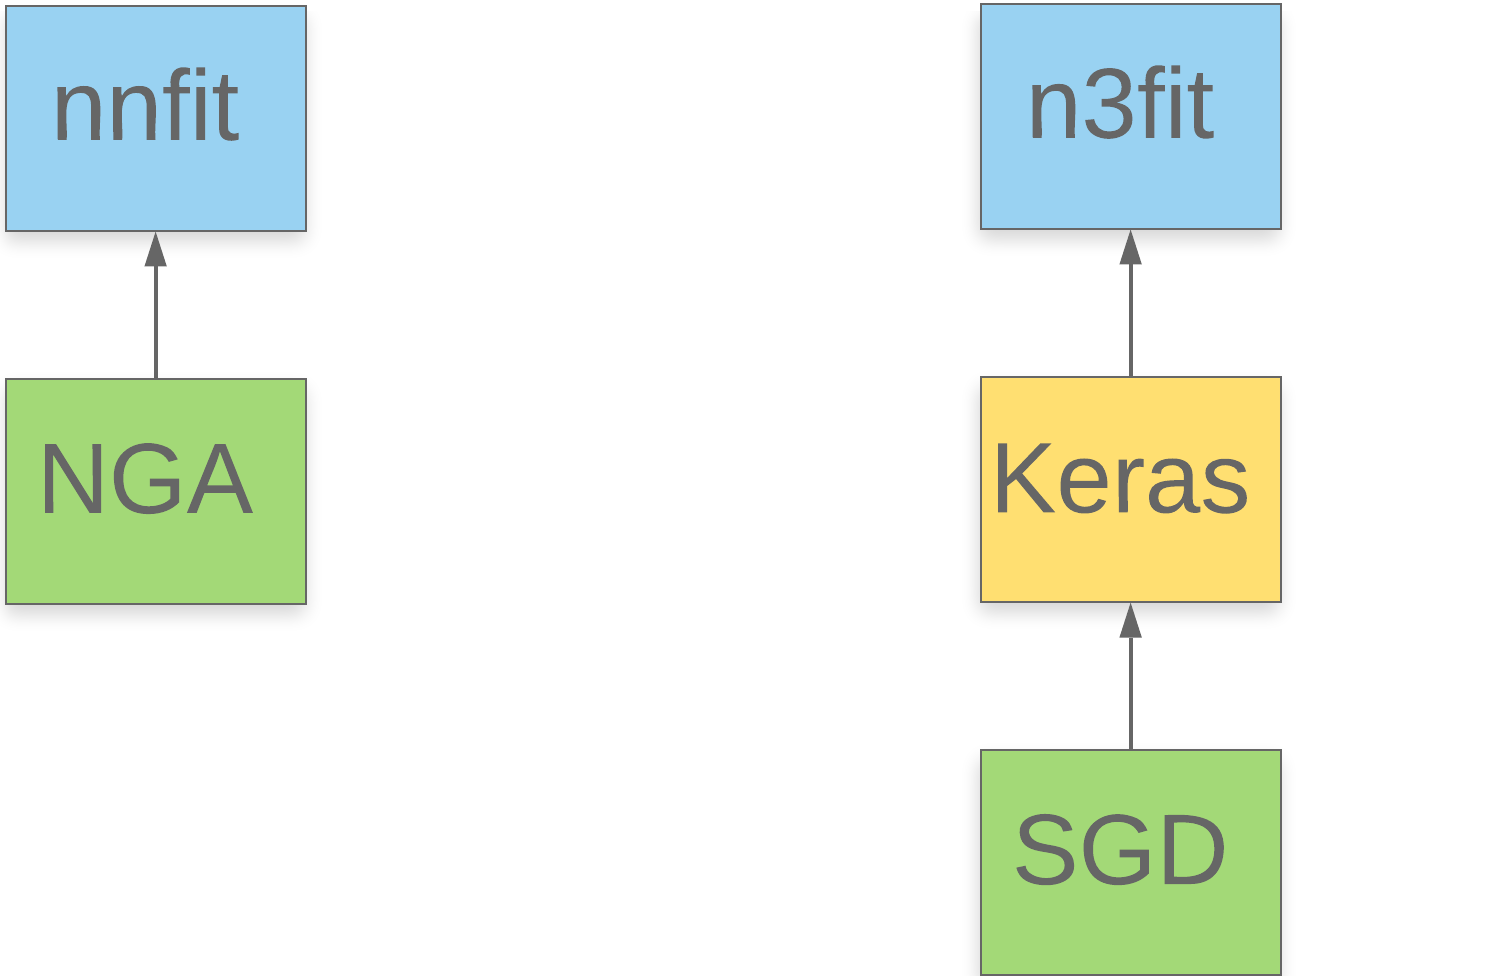
\includegraphics[height=135pt]{situation_before.png}
    \end{figure}
    }
    
    \only<2>{
    \begin{figure}
        \centering
        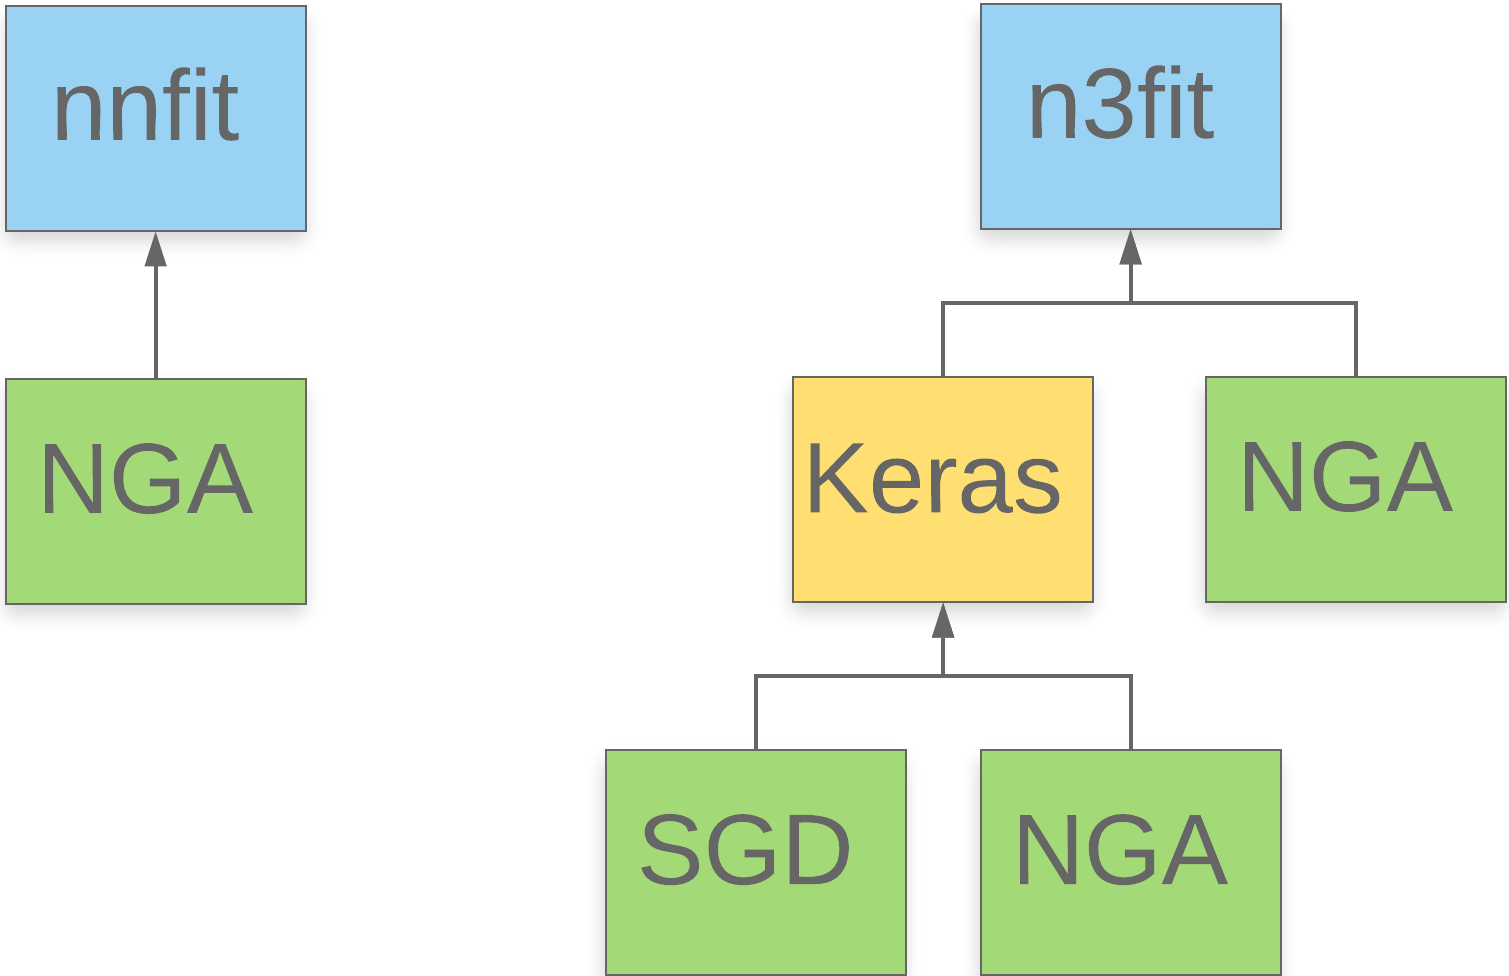
\includegraphics[height=135pt]{both_options.png}
    \end{figure}
    }
    
    \only<3>{
    \begin{figure}
        \centering
        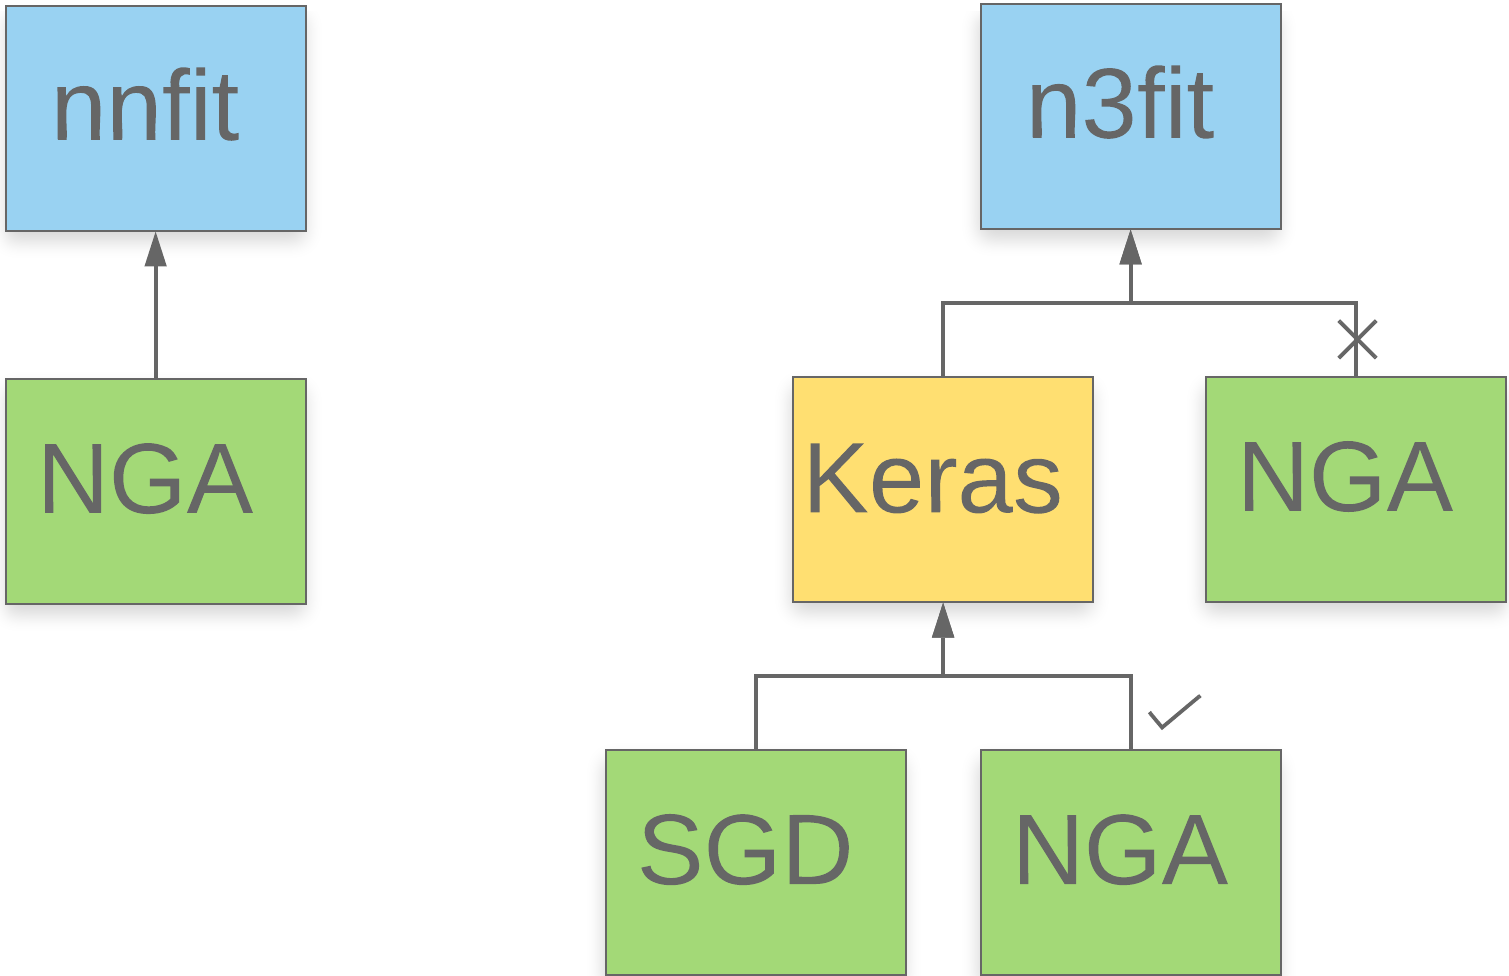
\includegraphics[height=135pt]{choice_made.png}
    \end{figure} 
    \texttt{evolutionary\_keras} is a general Keras library!
    }
\end{frame}


\begin{frame}[fragile]{Example}

Just replace Keras' Model by our EvolModel:
\vspace*{-10pt}
\begin{columns}[onlytextwidth]
\column{0.475\textwidth}
\lstset{emph={EvolModel, evolutionary_keras},emphstyle={\bfseries\underline}}
\begin{lstlisting}[language=Python, basicstyle=\tiny]
from evolutionary_keras.models import EvolModel

# prepare training and validation data
# prepare model using keras functional API

model = EvolModel(inputs, outputs)

model.compile(optimizer="nga", ... )

history = model.fit(...)
score = model.evaluate(...)
\end{lstlisting} 

\column{0.05\textwidth}
\column{0.475\textwidth}
\lstset{emph={Model, keras},emphstyle={\bfseries\underline}}
\begin{lstlisting}[language=Python, basicstyle=\tiny]
from keras.models import Model

# prepare training and validation data
# prepare model using keras functional API

model = Model(inputs, outputs)

model.compile(optimizer="rmsprop", ... )

history = model.fit(...)
score = model.evaluate(...)
\end{lstlisting} 
\end{columns}

\texttt{evolutionary\_keras} currently supports NGA and CMA-ES, \\ 
but other minimizers can be plugged in with relative ease \\
\end{frame}



\begin{frame}{Availability}
Docs: \href{http://evolutionary-keras.readthedocs.io/en/latest/}{\bulurl{evolutionary-keras.readthedocs.io/en/latest/}}\\
GitHub: \href{http://www.github.com/N3PDF/evolutionary_keras}{\bulurl{github.com/N3PDF/evolutionary_keras}}\\
PyPi: \texttt{pip install evolutionary-keras}\\
Conda: \texttt{conda install evolutionary\_keras}

\vspace{15pt}
\begin{columns}[onlytextwidth]
\column{0.475\textwidth}\centering
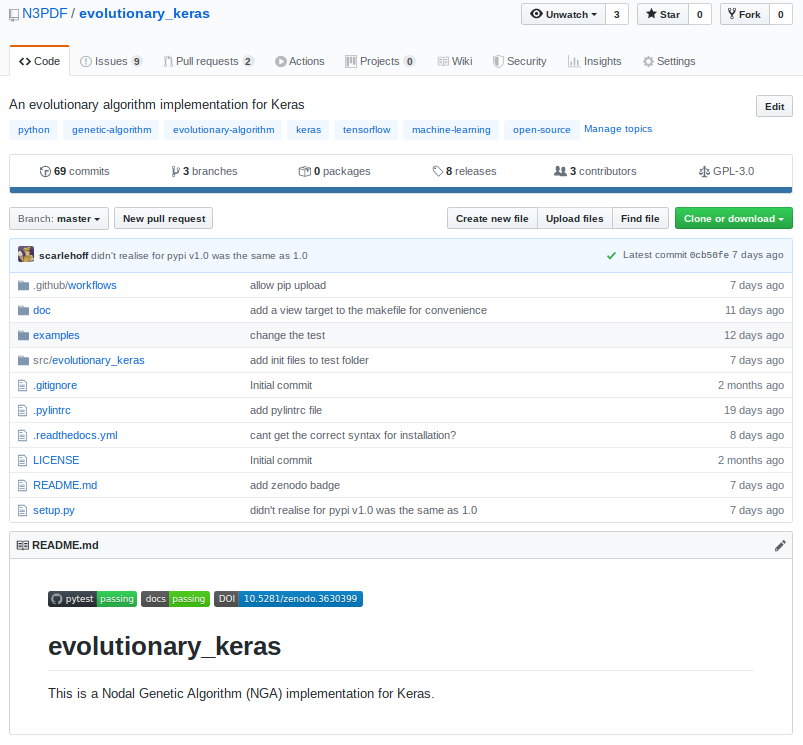
\includegraphics[height=130pt]{Screenshot_github.png}  
\column{0.05\textwidth}
\column{0.475\textwidth}\centering
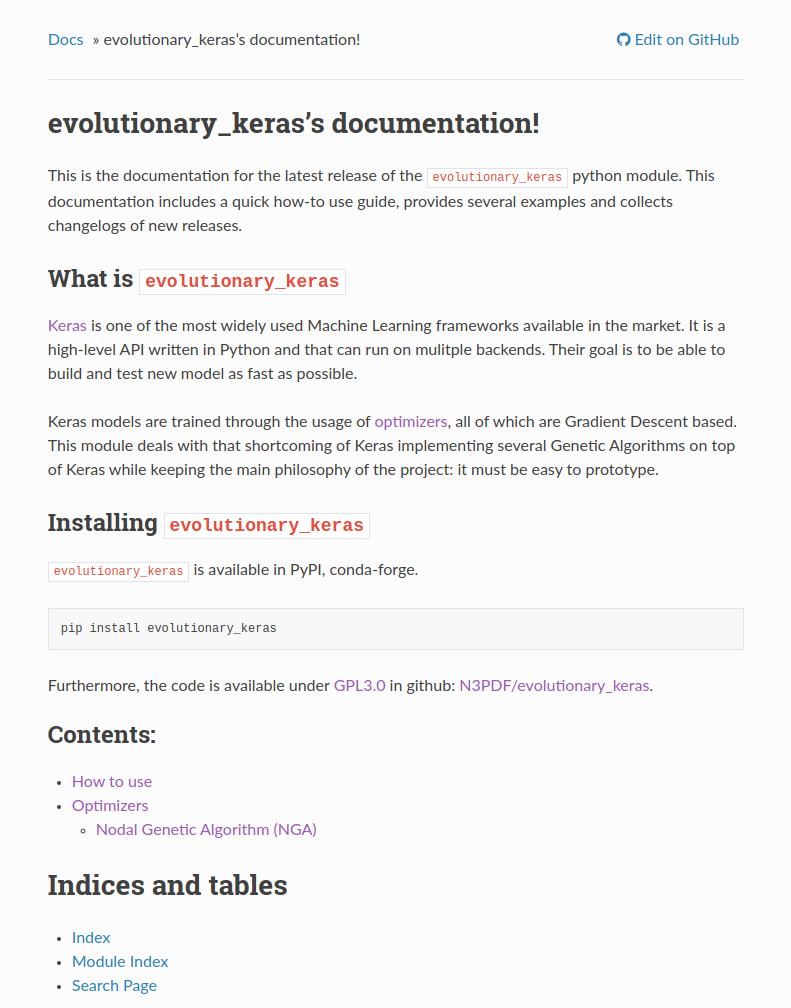
\includegraphics[height=130pt]{screenshot_readthedocs.png}
\end{columns}

%\begin{figure}
%    \centering
%    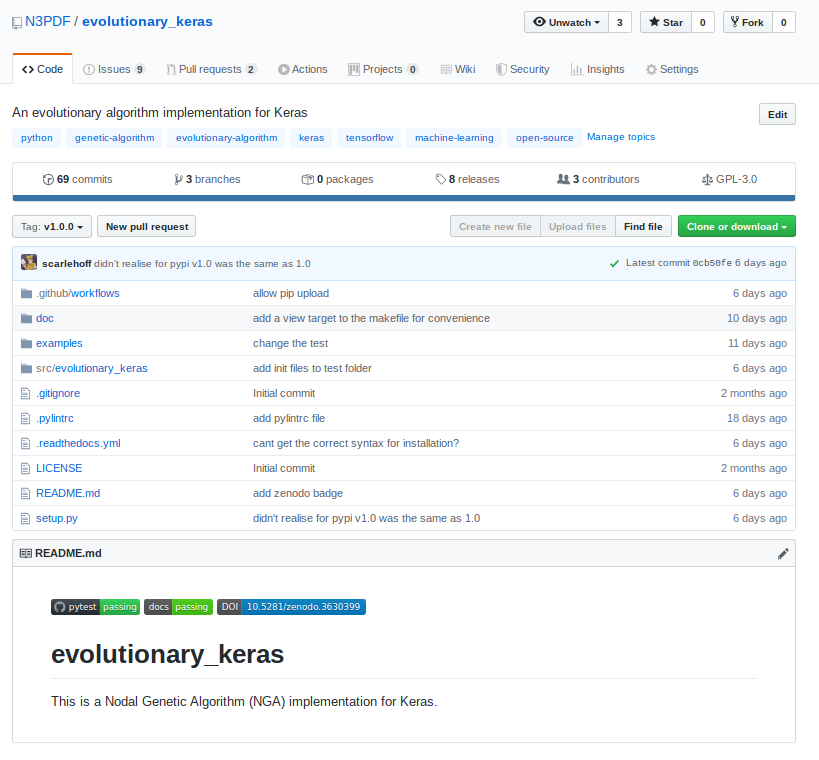
\includegraphics[height=120pt]{github.png}
%\end{figure}

\end{frame}

\section{PDF fits}

\begin{frame}{Global fit with \texttt{n3fit} and NGA}
\vspace{15pt}
\begin{center}
  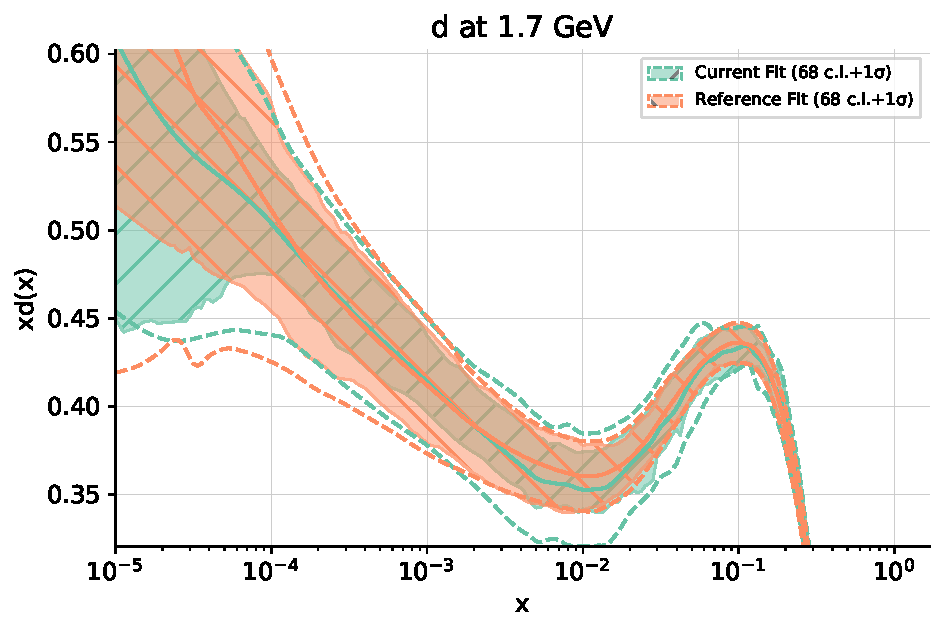
\includegraphics[width=0.7\textwidth]{Global_n3fit_NGA.pdf}  \\
{\centering\href{https://vp.nnpdf.science/KosxK7QHR0iBl2v21cVWpQ==}{\bulurl{vp.nnpdf.science/KosxK7QHR0iBl2v21cVWpQ==}}}
\end{center}
\end{frame}

\renewcommand{\appendixname}{\texorpdfstring{\translate{Appendix}}{Appendix}}
%\appendix


\begin{frame}{DIS fit with \texttt{n3fit} selected hyperparameters}
\vspace{15pt}
\begin{columns}[onlytextwidth]
\column{0.475\textwidth}
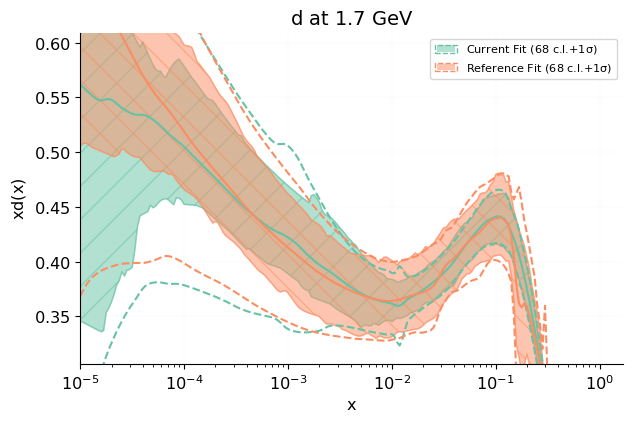
\includegraphics[width=\textwidth]{DIS_NNFITvsN3FIT_GAonly.png} \\
\hspace{0mm} \href{http://vp.nnpdf.science/yWw6yZRERZaCu3kbd96psg==/}{\color{blue} \underline{nnfit and n3fit both with NGA}} \\ 
{\hspace*{5mm}\tiny green is \texttt{n3fit}, orange is \texttt{nnfit}}
\column{0.05\textwidth}
\column{0.475\textwidth}
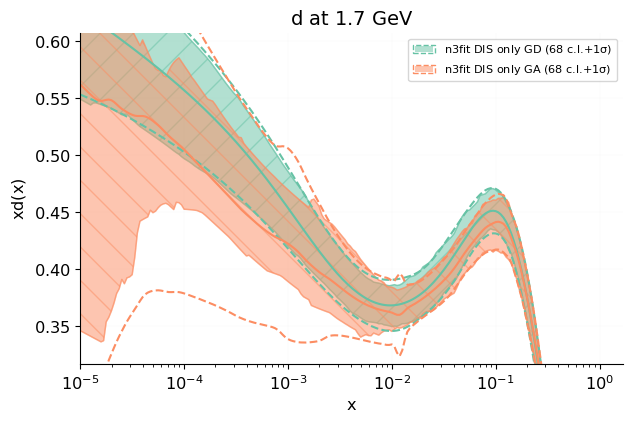
\includegraphics[width=\textwidth]{DIS_N3FIT_GAvsSGD.png} \\
\hspace{5mm} \href{http://vp.nnpdf.science/kxAUcKA5QX-4nD_gECTfiQ==/}{\color{blue} \underline{n3fit with NGA and SGD}}

\end{columns}

\end{frame}

\note[itemize]{
\item nnfit and n3fit both with NGA: http://vp.nnpdf.science/yWw6yZRERZaCu3kbd96psg==/
\item n3fit with NGA and SGD: http://vp.nnpdf.science/kxAUcKA5QX-4nD_gECTfiQ==/
}
